% !TeX root = ../../main.tex
\section{Technology Stack}\label{section:technology-stack}

Since most of the existing software for \ac{UBII} was written in \acf{JS}\footnote{\ac{JS} is a just-in-time compiled scripting language, widely used in web technology. It is a dynamic prototype-based language, which supports object-orientated programming.} using a fully web-based architecture, I decided to adapt this approach. This has one major advantage: platform independence. Most modern devices can run web-based software, which means they can also run our software. Also the software is served by a web server, which means the user does not have to install the software onto his device.

A web interface with some \ac{UBII} content (the \ac{UBII} front end), demos and debugging tools was already written, so I included my demos in this interface as well. The interface uses Vue.js as web framework.

\subsection{Vue.js}\label{subsection:vuejs}
Vue.js\footnote{Official Website: \href{https://vuejs.org/}{www.vuejs.org}} is a modern \ac{JS} web framework\footnote{A web framework is a software framework which provides a standard way to build web applications. It comes with tools and libraries to automate and make the development of web applications easier.}. Being released in 2014 and developed by Evan You~\cite[17]{Koetsier.2016}, it is a relatively young framework. But it quickly gained traction and is quite popular now~\cite[12\psq]{Koetsier.2016}.
Modules like Vue.js itself, Vue.js plugins and other JavaScript libraries are managed using the package manager npm~\footnote{Npm stands for \enquote{Node Package Manager} and is also used in the~\ac{UBII} server itself. Official website: \href{https://www.npmjs.com/}{www.npmjs.com}}.

\begin{figure}[htpb]
    \centering
    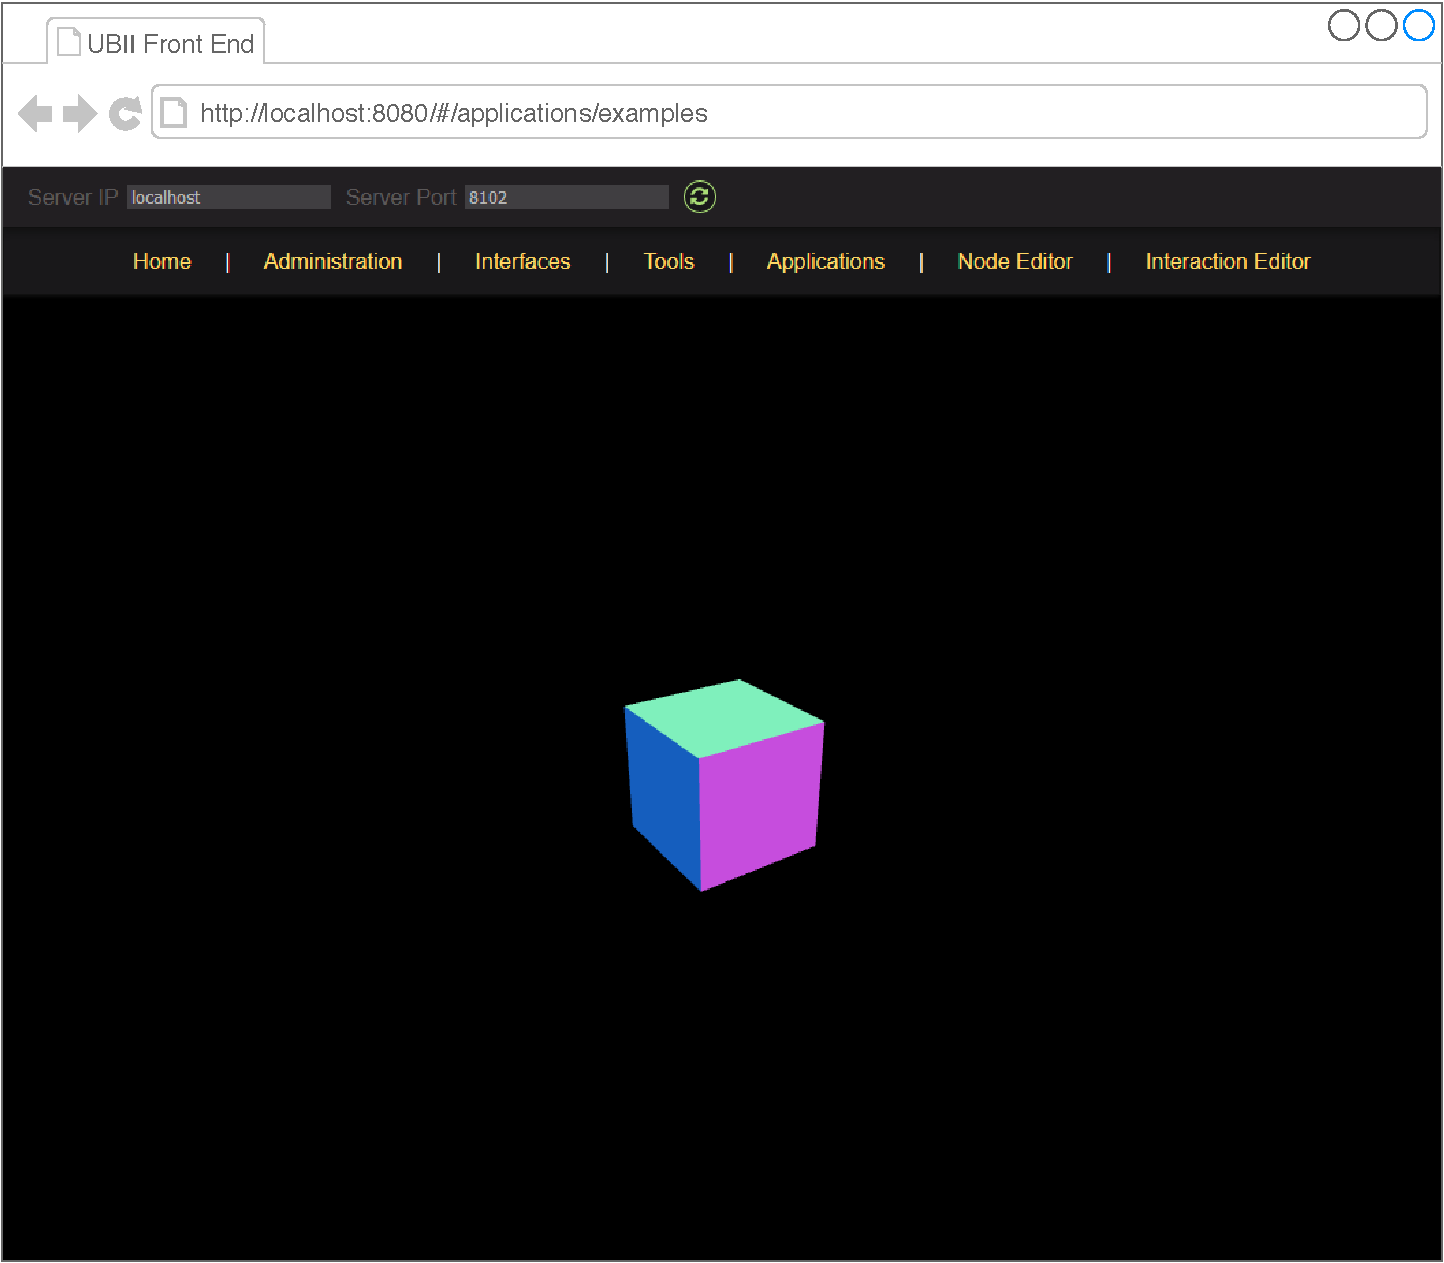
\includegraphics[width=12cm]{figures/ubii_front_end.pdf}
    \caption[The UBII Front End]{A screenshot of the UBII front end which was developed by Sandro Weber, Daniel Dyrda and me.}\label{fig:ubii_front_end}
  \end{figure}

The~\ac{UBII} front end has multiple Vue components for 